\subsection{Iterazioni di punto fisso}

\begin{examplebox}[: esempio di introduzione]
    Con una calcolatrice si può facilmente verificare che applicando ripetutamente la funzione $\cos$ partendo dal numero $1$ si genera la seguente successione di numeri reali:
    \begin{equation*}
        \begin{array}{lclcl}
            x^{\left(1\right)}  &=& \cos\left(1\right)                  &=& 0.54030230586814 \\ [1em]
            x^{\left(2\right)}  &=& \cos\left(x^{\left(1\right)}\right) &=& 0.85755321584639 \\
            \vdots              & &                                     & & \\
            x^{\left(10\right)} &=& \cos\left(x^{\left(9\right)}\right) &=& 0.74423735490056 \\
            \vdots              & &                                     & & \\
            x^{\left(20\right)} &=& \cos\left(x^{\left(19\right)}\right)&=& 0.73918439977149
        \end{array}
    \end{equation*}
    Che tende al valore $\alpha = 0.73908513$.
\end{examplebox}

\noindent
Con l'esempio di introduzione è possibile capire il punto fisso. Essendo per costruzione $x^{\left(k+1\right)} = \cos\left(x^{\left(k\right)}\right)$ per $k = 0, 1, \dots$ (con $x^{\left(0\right)} = 1$), $\alpha$ è tale che $\cos\left(\alpha\right) = \alpha$. Quindi, $\alpha$ viene detto punto fisso della funzione coseno.

\highspace
\begin{flushleft}
    \textcolor{Green3}{\faIcon{question-circle} \textbf{Perché è interessante?}}
\end{flushleft}
Se $\alpha$ è un punto fisso per il coseno, allora esso è uno zero della funzione $f\left(x\right) = x - \cos\left(x\right)$ ed il metodo appena proposto potrebbe essere usato per il calcolo degli zeri di $f$.

\highspace
\begin{flushleft}
    \textcolor{Red2}{\faIcon{exclamation-triangle} \textbf{Non tutte le funzioni hanno un punto fisso}}
\end{flushleft}
Non tutte le funzioni ammettono punti fissi. Ad esempio, ripetendo l'esperimento dell'esempio con una funzione esponenziale a partire da $x^{\left(0\right)} = 1$, dopo soli 4 passi si giunge ad una situazione di \emph{overflow} (figura \ref{fig: non tutte le funzioni hanno un punto fisso}, pagina \pageref{fig: non tutte le funzioni hanno un punto fisso}).

\begin{definitionbox}
    Data una funzione $\phi: \left[a, b\right] \rightarrow \mathbb{R}$, trovare $\alpha \in \left[a,b\right]$ tale che:
    \begin{equation*}
        \alpha = \phi\left(\alpha\right)
    \end{equation*}
    Se tale $\alpha$ esiste, viene detto un \definition{punto fisso} di $\phi$ e lo si può determinare come limite della seguente successione:
    \begin{equation}
        x^{\left(k+1\right)} = \phi\left(x^{\left(k\right)}\right) \hspace{2em} k \ge 0
    \end{equation}
    Dove $x^{\left(0\right)}$ è un dato iniziale. L'algoritmo viene chiamato \definition{iterazioni di punto fisso} e la funzione $\phi$ è detta \definition{funzione di iterazione}.
\end{definitionbox}

\noindent
Dalla definizione, si deduce che l'esempio introduttivo è un algoritmo di iterazioni di punto fisso per la funzione $\phi\left(x\right) = \cos\left(x\right)$.

\newpage

\begin{figure}[!htp]
    \centering
    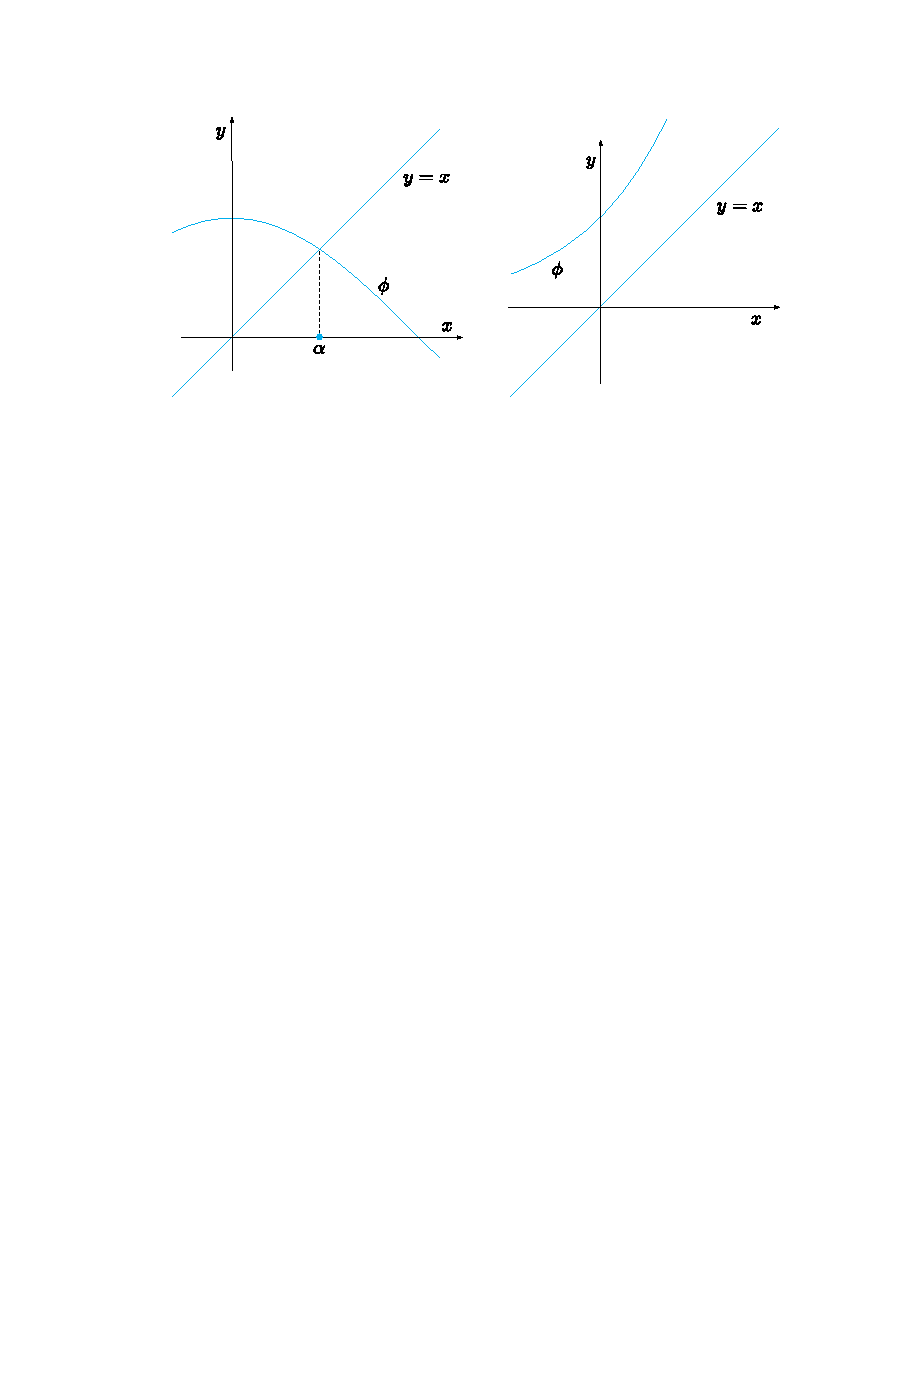
\includegraphics[width=\textwidth]{img/iterazioni-di-punto-fisso-1.pdf}
    \caption{La funzione $\phi\left(x\right) = \cos\left(x\right)$ (sx) ammette un solo punto fisso, mentre la funzione $\phi\left(x\right) = e^{x}$ (dx) non ne ammette alcuno.}
    \label{fig: non tutte le funzioni hanno un punto fisso}
\end{figure}

\begin{figure}[!htp]
    \centering
    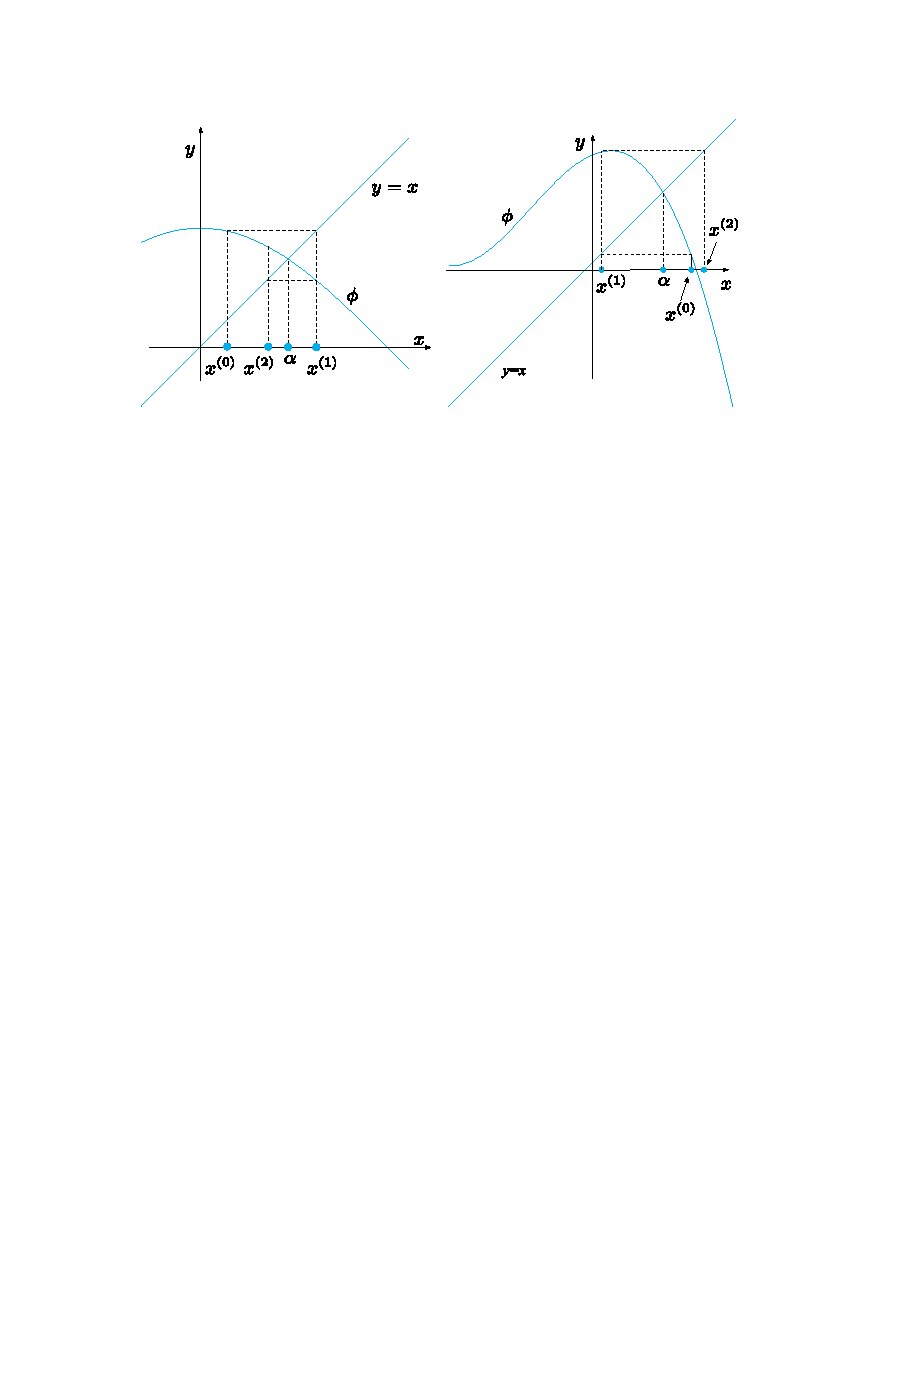
\includegraphics[width=\textwidth]{img/iterazioni-di-punto-fisso-2.pdf}
    \caption{Rappresentazione delle prime iterazioni di punto fisso per due funzioni di iterazione. Le iterazioni convergono verso il punto fisso $\alpha$ (sx), mentre si allontanano da $\alpha$ (dx).}
    \label{fig: interpretazione geometrica di un punto fisso}
\end{figure}